\documentclass[a4paper]{article}
\usepackage[utf8x]{inputenc}
\usepackage[T1,T2A]{fontenc}
\usepackage[russian]{babel}
\usepackage{hyperref}
\usepackage{indentfirst}
\usepackage{color}
\usepackage{listings}
\usepackage{here}
\usepackage{array}
\usepackage{multirow}
\usepackage{graphicx}
\usepackage{caption}

\lstset{ %
extendedchars=\true,
keepspaces=true,
language=C++,					% choose the language of the code
basicstyle=\footnotesize,		% the size of the fonts that are used for the code
numbers=left,					% where to put the line-numbers
numberstyle=\footnotesize,		% the size of the fonts that are used for the line-numbers
stepnumber=1,					% the step between two line-numbers. If it is 1 each line will be numbered
numbersep=5pt,					% how far the line-numbers are from the code
backgroundcolor=\color{white},	% choose the background color. You must add \usepackage{color}
showspaces=false				% show spaces adding particular underscores
showstringspaces=false,			% underline spaces within strings
showtabs=false,					% show tabs within strings adding particular underscores
frame=single,           		% adds a frame around the code
tabsize=4,						% sets default tabsize to 2 spaces
captionpos=b,					% sets the caption-position to bottom
breaklines=true,				% sets automatic line breaking
breakatwhitespace=false,		% sets if automatic breaks should only happen at whitespace
escapeinside={\%*}{*)},			% if you want to add a comment within your code
postbreak=\raisebox{0ex}[0ex][0ex]{\ensuremath{\color{red}\hookrightarrow\space}}
}
\begin{document}	% начало документа


\begin{titlepage}	% начало титульной страницы

	\begin{center}		% выравнивание по центру

		\large Санкт-Петербургский Политехнический Университет Петра Великого\\
		\large Институт компьютерных наук и технологий \\
		\large Кафедра компьютерных систем и программных технологий\\[6cm]
		% название института, затем отступ 6см
		
		\huge Программирование\\[0.5cm] % название работы, затем отступ 0,5см
		\large Отчет по курсовой работе\\[0.1cm]
		\large "Шашки"\\[5cm]

	\end{center}


	\begin{flushright} % выравнивание по правому краю
		\begin{minipage}{0.25\textwidth} % врезка в половину ширины текста
			\begin{flushleft} % выровнять её содержимое по левому краю

				\large\textbf{Работу выполнил:}\\
				\large Корсков А.В.\\
				\large {Группа:} 23501/4\\
				
				\large \textbf{Преподаватель:}\\
				\large Вылегжанина К.Д.
				

			\end{flushleft}
		\end{minipage}
	\end{flushright}
	
	\vfill % заполнить всё доступное ниже пространство

	\begin{center}
	\large Санкт-Петербург\\
	\large \the\year % вывести дату
	\end{center} % закончить выравнивание по центру

\thispagestyle{empty} % не нумеровать страницу
\end{titlepage} % конец титульной страницы

\vfill % заполнить всё доступное ниже пространство
% Содержание
\tableofcontents
\newpage

\section{Игра Шашки}
\subsection{Задание}
У нас имеется прямоугольное поле размером 8х8, которое окрашено в чёрный и белый цвет. На этом поле расставленны шашки. Два игрока по очереди передвигают свои шашки. Целью игры является уничтожение всех шашек соперника. У кого шашек не осталось, тот и считается проигравшим.

\subsection{Правила работы программы}
Всё действие происходит на поле размером 8х8. Во время партии каждому игроку принадлежат шашки одного цвета: чёрного или белого. Цель игры — лишить противника возможности хода путём взятия или запирания всех его шашек. Все шашки, участвующие в партии, выставляются перед началом игры на доску. Далее они передвигаются по полям доски и могут быть сняты с неё в случае боя шашкой противника.Брать шашку, находящуюся под боем, обязательно.Существует только два вида шашек: простые и дамки. В начале партии все шашки простые. Простая шашка может превратиться в дамку, если она достигнет последнего противоположного горизонтального ряда доски (дамочного поля).Простые шашки ходят только вперёд на следующее поле. Дамки могут ходить и вперёд и назад.

\subsection{Концепция}
Готовый проект должен моделировать игру между двумя игроками в шашки. Пользователь должен иметь возможность наблюдать за текущим состоянием игры, передвигать шашки и бить шашки противника. 

\subsection{Минимально работоспособный продукт}
Минимально работоспособный продукт должен уметь: предоставить пользователю информацию о текущем состоянии игры, давать игроку возможность передвигать свои шашки, уничтожать шашки противника.


\subsection{Диаграмма прецедентов использования}

\begin{figure}[H]
	\begin{center}
		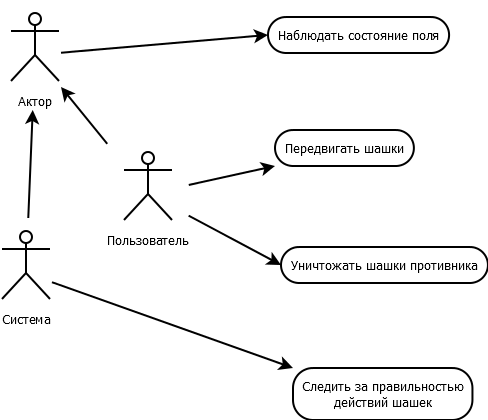
\includegraphics[scale=0.4, height=7cm]{Diagram1}
		\caption{Диаграмма прецедентов использования} 
		\label{pic:Diagram1} % название для ссылок внутри кода
	\end{center}
\end{figure}

\section{Проектрование приложения, реализующего игру Шашки}

\subsection{Библиотека}
При написании проекта, была создана библиотека. В ней находятся все необходимые классы для создания и работы игры. Один из классов (api) создан для предоставления всех действий над моделью.

\noindent В API выделены следующие методы: 
\begin{itemize}
\item move\_draught - метод, передвигающий шашку.
\item destroy\_draught - метод, уничтожающий шашку противника.
\item get\_statistics - метод, анализирующий поле и выдающий статистику.
\item check\_destruction\_around - метод, проверяющий может ли шашка кого-нибудь уничтожить вокруг себя.
\end{itemize}


\section{Реализация игры Шашки}
\subsection{Версии программ}
Операционная система: Windows 8, среда разработки: Android Studio 2.3, компилятор: Gradle 3.0, Java 1.8.0.120.

\subsection{Библиотека}
\noindent Основные классы, выделенные в библиотеке:
\begin{itemize}
\item Класс Draughts. Реализует шашку. Содержит координаты шашки, её цвет и тип. Присутствуют методы, возвращающие и задающие координаты и состояние шашки, проверяющий может ли данная шашка сделать заданный ход и ещё один метод, проверяющий достигла ли шашка концаа поля.
\item Класс Field. Класс представляет поле игры. Содержит двумерный массив клеток и цвет текущего хода. Присутствуют методы, возвращающие и задающие двумерном массиве и цвет текущего хода, также есть методы: проверяющий свободна ли данная клетка и проверяющий  может ли она уничтожить данную шашку противника.	
\item Класс Api. Класс, предоставляющий все методы, доступные над игрой. Позволяет сделать ход шашкой, уничтожить шашку противника, сохранить поле в файл, загрузить поле из файла, получить данные о текущем состоянии поля и метод, узнающий может ли шашка уничтожить кого-нибудь вокруг себя
\end{itemize}

\subsection{Андроид приложение}
Андроид приложение позволяет играть на устройствах под управлением ОС Андроид.

\noindent Основные классы, выделенные в Андроид приложении. 
\begin{itemize}
\item Класс About. Класс, который выводит информацию о правилах игры.
\item Класс Draught. Главное меню приложение. В этом классе расположены кнопки: "Новая игра", "Помощь", "Выход".
\item Класс DraughtView. Класс отвечающий за отрисовку поля. Все действия над полем происходят именно в этом классе.
\item Класс Game. Класс, который вызывает отрисовку поля. Также он выводит сообщения о неправильных действиях игрока.
\item Класс Music. Класс отвечающий за воспроизводство музыки. В нём можно запускать и останавливать проигрывание аудио файла.
\end{itemize}

\begin{figure}[H]
	\begin{center}
		\includegraphics[scale=0.5]{gui}
		\caption{Главное меню графического приложения} 
		\label{pic:menu} % название для ссылок внутри кода
	\end{center}
\end{figure}

На рис \ref{pic:menu} представлено главное окно приложения. В нём пользователю можно начать играть, открыть помощь или выйти. 

\begin{figure}[H]
	\begin{center}
		\includegraphics[scale=0.5]{gui2}
		\caption{Представление поля в графическом приложении} 
		\label{pic:field} % название для ссылок внутри кода
	\end{center}
\end{figure}

На рис \ref{pic:field} – окно с полем. В центре расположено поле с шашками, внизу текущие данные об игре для каждой из сторон и информация о том, чей ход в данный момент.

\section{Процесс обеспечения качества и тестирование}
\subsection{Тестирование}
Приложение тестировалось вручную. После добавления каждой новой функции в приложение, она была протестирована на работоспособность. После теста при возникновении ошибок они все были исправлены.

\section{Вывод}
По окончании семестра автор проекта научился писать программы на языке Java для операционной системы Android, делать графический интерфейс с помощью Swing, а также получил опыт работы с большими проектами на Java, содержащими много классов и имеющих как консольное приложение, так и графическое.

\section{Приложение 1. Листинги кода}
\subsection{Консольное приложение}
\lstinputlisting[]
{../Draughts/src/main/java/ConsoleApp/Console_Ui.java}
\newpage

\subsection{Графическое приложение}
\lstinputlisting[]
{../Draughts/src/main/java/Graphic_Ui/Frame.java}
\newpage

\lstinputlisting[]
{../Draughts/src/main/java/Graphic_Ui/Board.java}
\newpage

\lstinputlisting[]
{../Draughts/src/main/java/Graphic_Ui/BorderPanel.java}
\newpage

\subsection{Библиотека}

\lstinputlisting[]
{../Draughts/src/main/java/Core/Api.java}
\newpage

\lstinputlisting[]
{../Draughts/src/main/java/Core/Draught.java}
\newpage

\lstinputlisting[]
{../Draughts/src/main/java/Core/Field.java}
\newpage

\subsection{Тесты}

\lstinputlisting[]
{../Draughts/src/test/java/Test_Draughts.java}
\newpage
\end{document}